\PassOptionsToPackage{unicode=true}{hyperref} % options for packages loaded elsewhere
\PassOptionsToPackage{hyphens}{url}
%
\documentclass[12pt,openright,oneside,a4paper,chapter=TITLE,section=TITLE,subsection=Title,english,french,spanish,portugues,sumario=tradicional]{04-class-files/abntex2}
\usepackage{lmodern}
\usepackage{amssymb,amsmath}
\usepackage{ifxetex,ifluatex}
\usepackage{fixltx2e} % provides \textsubscript
\ifnum 0\ifxetex 1\fi\ifluatex 1\fi=0 % if pdftex
  \usepackage[T1]{fontenc}
  \usepackage[utf8]{inputenc}
  \usepackage{textcomp} % provides euro and other symbols
\else % if luatex or xelatex
  \usepackage{unicode-math}
  \defaultfontfeatures{Ligatures=TeX,Scale=MatchLowercase}
\fi
% use upquote if available, for straight quotes in verbatim environments
\IfFileExists{upquote.sty}{\usepackage{upquote}}{}
% use microtype if available
\IfFileExists{microtype.sty}{%
\usepackage[]{microtype}
\UseMicrotypeSet[protrusion]{basicmath} % disable protrusion for tt fonts
}{}
\IfFileExists{parskip.sty}{%
\usepackage{parskip}
}{% else
\setlength{\parindent}{0pt}
\setlength{\parskip}{6pt plus 2pt minus 1pt}
}
\usepackage{hyperref}
\hypersetup{
            pdfauthor={Jackson da Silva Torres},
            pdfborder={0 0 0},
            breaklinks=true}
\urlstyle{same}  % don't use monospace font for urls
\usepackage{longtable,booktabs}
% Fix footnotes in tables (requires footnote package)
\IfFileExists{footnote.sty}{\usepackage{footnote}\makesavenoteenv{longtable}}{}
\usepackage{graphicx,grffile}
\makeatletter
\def\maxwidth{\ifdim\Gin@nat@width>\linewidth\linewidth\else\Gin@nat@width\fi}
\def\maxheight{\ifdim\Gin@nat@height>\textheight\textheight\else\Gin@nat@height\fi}
\makeatother
% Scale images if necessary, so that they will not overflow the page
% margins by default, and it is still possible to overwrite the defaults
% using explicit options in \includegraphics[width, height, ...]{}
\setkeys{Gin}{width=\maxwidth,height=\maxheight,keepaspectratio}
\setlength{\emergencystretch}{3em}  % prevent overfull lines
\providecommand{\tightlist}{%
  \setlength{\itemsep}{0pt}\setlength{\parskip}{0pt}}
\setcounter{secnumdepth}{5}
% Redefines (sub)paragraphs to behave more like sections
\ifx\paragraph\undefined\else
\let\oldparagraph\paragraph
\renewcommand{\paragraph}[1]{\oldparagraph{#1}\mbox{}}
\fi
\ifx\subparagraph\undefined\else
\let\oldsubparagraph\subparagraph
\renewcommand{\subparagraph}[1]{\oldsubparagraph{#1}\mbox{}}
\fi

% set default figure placement to htbp
\makeatletter
\def\fps@figure{htbp}
\makeatother

%%%%%%%%%%%%%%%%%%%%%%%%%%%%%%%%%%%%%%%%%%%%%%%%%%%%%%%
% Arquivo para entrada de dados para a parte pré textual
%%%%%%%%%%%%%%%%%%%%%%%%%%%%%%%%%%%%%%%%%%%%%%%%%%%%%%%
% 
% Basta digitar as informações indicidas, no formato 
% apresentado.
%
%%%%%%%
% Os dados solicitados são, na ordem:
%
% tipo do trabalho
% componentes do trabalho 
% título do trabalho
% nome do autor
% local 
% data (ano com 4 dígitos)
% orientador(a)
% coorientador(a)(as)(es)
% arquivo com dados bibliográficos
% instituição
% setor
% programa de pós gradução
% curso
% preambulo
% data defesa
% CDU
% errata
% assinaturas - termo de aprovação
% resumos & palavras chave
% agradecimentos
% dedicatoria
% epígrafe


% Informações de dados para CAPA e FOLHA DE ROSTO
%----------------------------------------------------------------------------- 
\tipotrabalho{Dissertação}

% Marcar Sim para as partes que irão compor o documento pdf
%----------------------------------------------------------------------------- 
 \providecommand{\terCapa}{Sim}
 \providecommand{\terFolhaRosto}{Sim}
 \providecommand{\terTermoAprovacao}{Nao}
 \providecommand{\terDedicatoria}{Nao}
 \providecommand{\terFichaCatalografica}{Nao}
 \providecommand{\terEpigrafe}{Nao}
 \providecommand{\terAgradecimentos}{Nao}
 \providecommand{\terErrata}{Nao}
 \providecommand{\terListaFiguras}{Sim}
 \providecommand{\terListaTabelas}{Sim}
 \providecommand{\terSiglasAbrev}{Nao}
 \providecommand{\terResumos}{Nao}
 \providecommand{\terSumario}{Sim}
 \providecommand{\terAnexo}{Nao}
 \providecommand{\terApendice}{Nao}
 \providecommand{\terIndiceR}{Nao}
%----------------------------------------------------------------------------- 

\titulo{Efeitos das variações dos componentes do \emph{Spread} na rentabilidade das instituições bancárias através da análise de dados em painel
}
\autor{}
\local{Curitiba}
\data{2020} %Apenas ano 4 dígitos

% Orientador ou Orientadora
\orientador{}
%Prof Emílio Eiji Kavamura, MSc}
\orientadora{
Prof\textordfeminine~Dra. Mayla Costa}
% Pode haver apenas uma orientadora ou um orientador
% Se houver os dois prevalece o feminino.

% Em termos de coorientação, podem haver até quatro neste modelo
% Sendo 2 mulhere e 2 homens.
% Coorientador ou Coorientadora
\coorientador{}%Prof Morgan Freeman, DSc}
\coorientadora{}

% Segundo Coorientador ou Segunda Coorientadora
\scoorientador{}
%Prof Jack Nicholson, DEng}
\scoorientadora{}
%Prof\textordfeminine~Ingrid Bergman, DEng}
% ----------------------------------------------------------
%\addbibresource{10-references/referencias.bib}
%\bibliography{10-references/referencias.bib}
% ----------------------------------------------------------
\instituicao{Universidade Federal do Paraná}

\def \ImprimirSetor{Departamento de Economia}%
%Setor de Tecnologia}

\def \ImprimirProgramaPos{Programa Profissional de Pós-Graduação em Economia}

\def \ImprimirCurso{Mestrado Profissional em Economia}

\preambulo{
Trabalho apresentado como requisito parcial para a obtenção do título de Mestre Profisisonal em Economia no curso de Mestrado Profissional em Economia pelo Departamento de Economia da Universidade Federal do Paraná}
%do grau de Bacharel em Expressão Gráfica no curso de Expressão Gráfica, Setor de Exatas da Universidade Federal do Paraná}

%----------------------------------------------------------------------------- 

\newcommand{\imprimirCurso}{}
%Programa de P\'os Gradua\c{c}\~ao em Engenharia da Constru\c{c}\~ao Civil}

\newcommand{\imprimirDataDefesa}{
31 de Dezembro de 2020}

\newcommand{\imprimircdu}{
02:141:005.7}

% ----------------------------------------------------------
\newcommand{\imprimirerrata}{

\vspace{\onelineskip}


\begin{table}[htb]
\center
\footnotesize
\begin{tabular}{|p{1.4cm}|p{1cm}|p{3cm}|p{3cm}|}
  \hline
   \textbf{Folha} & \textbf{Linha}  & \textbf{Onde se lê}  & \textbf{Leia-se}  \\
    \hline
    1 & 10 & auto-conclavo & autoconclavo\\
   \hline
\end{tabular}
\end{table}}

% Comandos de dados - Data da apresentação
\providecommand{\imprimirdataapresentacaoRotulo}{}
\providecommand{\imprimirdataapresentacao}{}
\newcommand{\dataapresentacao}[2][\dataapresentacaoname]{\renewcommand{\dataapresentacao}{#2}}

% Comandos de dados - Nome do Curso
\providecommand{\imprimirnomedocursoRotulo}{}
\providecommand{\imprimirnomedocurso}{}
\newcommand{\nomedocurso}[2][\nomedocursoname]
  {\renewcommand{\imprimirnomedocursoRotulo}{#1}
\renewcommand{\imprimirnomedocurso}{#2}}


% ----------------------------------------------------------
\newcommand{\AssinaAprovacao}{

\assinatura{%\textbf
   {Professora} \\ UFPR}
   \assinatura{%\textbf
   {Professora} \\ ENSEADE}
   \assinatura{%\textbf
   {Professora} \\ TIT}
   %\assinatura{%\textbf{Professor} \\ Convidado 4}
      
   \begin{center}
    \vspace*{0.5cm}
    %{\large\imprimirlocal}
    %\par
    %{\large\imprimirdata}
    \imprimirlocal, \imprimirDataDefesa.
    \vspace*{1cm}
  \end{center}
  }
  
% ----------------------------------------------------------
%\newcommand{\Errata}{%\color{blue}
%Elemento opcional da \textcite[4.2.1.2]{NBR14724:2011}. Exemplo:
%}

% ----------------------------------------------------------
\newcommand{\EpigrafeTexto}{%\color{blue}
\textit{Texto}
}

% ----------------------------------------------------------
\newcommand{\ResumoTexto}{%\color{blue}

}

\newcommand{\PalavraschaveTexto}{%\color{blue}
latex. abntex. editoração de texto.}

% ----------------------------------------------------------
\newcommand{\AbstractTexto}{%\color{blue}
This is the english abstract.
}
% ---
\newcommand{\KeywordsTexto}{%\color{blue}
latex. abntex. text editoration.
}

% ----------------------------------------------------------
\newcommand{\Resume}
{%\color{blue}
Il s'agit d'un résumé en français.
} 
% ---
\newcommand{\Motscles}
{%\color{blue}
 latex. abntex. publication de textes.
}

% ----------------------------------------------------------
\newcommand{\Resumen}
{%\color{blue}
Este es el resumen en español.
}
% ---
\newcommand{\Palabrasclave}
{%\color{blue}
latex. abntex. publicación de textos.
}

% ----------------------------------------------------------
\newcommand{\AgradecimentosTexto}{%\color{blue}

}

% ----------------------------------------------------------
\newcommand{\DedicatoriaTexto}{%\color{blue}
\textit{}
	}


%\usepackage{geometry}


% Pacotes básicos 
% ----------------------------------------------------------
%\usepackage{lmodern}			% Usa a fonte Latin Modern			
\usepackage[utf8]{inputenc}		% Codificacao do documento (conversão automática dos acentos)
\usepackage{csquotes}
\usepackage[T1]{fontenc}		% Selecao de codigos de fonte.
\usepackage{lastpage}			% Usado pela Ficha catalográfica
\usepackage{indentfirst}		% Indenta o primeiro parágrafo de cada seção.
\usepackage{color}		    	% Controle das cores
\usepackage{graphicx}			% Inclusão de gráficos
\usepackage{microtype} 			% para melhorias de justificação
\usepackage{ifthen}		    	% para montar condicionais
%\usepackage[brazil]{babel}		% para utilizar termos em portugues
\usepackage[final]{pdfpages}    % para incluir páginas de arquivos pdf
\usepackage{lipsum}				% para geração de dummy text
\usepackage{csquotes}

%\usepackage[style=long]{glossaries}
%\usepackage{abntex2glossaries}

% permite representar o cancelamento de termos em texto ou equacoes
\usepackage{cancel} 		
% cores extendidas
\usepackage{xcolor} 		
% gera diagramas a partir de listas
\usepackage{smartdiagram}   
% Para a figura ficar na posição correta
\usepackage{float} 		    
% supporte para fontes da Text Companion 
\usepackage{textcomp} 		
% uso de longtable
\usepackage{longtable}		
% simbolos matematicos
\usepackage{amsmath}	
% páginas em paisagem
\usepackage{lscape}
% mescla de colunas em tabelas
\usepackage{multicol}
% mescla de linhas em tabelas
\usepackage{multirow}
% criação do indice de quadros
\usepackage{newfloat} 
% configura legenda 
\usepackage{caption} 		
%[format=plain]
	%\renewcommand\caption[1]{%
    \captionsetup{font=small}	% tamanho da fonte 10pt
    %,format=hang
 	% \caption{#1}}
	%\captionsetup{width=0.8\textwidth}
	
%\usepackage{scrpage2}

% Pacotes de citações BibLaTeX
% ----------------------------------------------------------
\usepackage[
style=abnt,
%backref=true,
backend=biber,
maxcitenames=3,
%citecounter=true,
%backrefstyle=three,
nohashothers=true
]{biblatex}


\DefineBibliographyStrings{brazil}{%
 backrefpage = {Citado \arabic{citecounter} vez na página},% originally "cited on page"
 backrefpages = {Citado \arabic{citecounter} vezes nas páginas},% originally "cited on pages"
}

% ----------------------------------------------------------

% alterando o aspecto da cor azul
\definecolor{blue}{RGB}{55,10,249}

% ----------------------------------------------------------
\PrepareListOf{quadro}{%
\renewcommand{\cftfigpresnum}{Quadro~}}

\DeclareFloatingEnvironment[
fileext=loq,
listname={\textbf{LISTA DE QUADROS}},
name=Quadro,
%placement=p,
within= none, % numeracao continua
%within=section, % numeracao reinicia em cada seccao
%chapterlistsgaps=off
]{quadro}

\newlistentry{quadro}{loq}{0}


% Customize ‘List of Diagrams’
\PrepareListOf{quadro}{%
\renewcommand{\cftquadropresnum}{\normalsize{QUADRO}~}
\setlength{\cftquadronumwidth}{3.2cm}
%\renewcommand{\cftquadroname}{\quadroname\space} 
\renewcommand*{\cftquadroaftersnum}{\hfill--\hfill}
}

\makeatletter
%% we define a helper macro for adjusting lists of new floats to
%% accept a * behind them for not being shown in the TOC, like
%% the other list printing commands in memoir
\newcommand{\AdjustForMemoir}[1]{%
  \csletcs{kept@listof#1}{listof#1}%
  \csdef{listof#1}{%
    \@ifstar
     {\csappto{newfloat@listof#1@hook}{\append@star}%
      \csuse{kept@listof#1}}%
     {\csuse{kept@listof#1}}%
  }
}
\def\append@star#1{#1*}
\makeatother


\AdjustForMemoir{quadro} % prepare `\listofdirfigures` so it accepts a *

\makeatletter
\let\oldcontentsline\contentsline
\def\contentsline#1#2{%
    \expandafter\ifx\csname l@#1\endcsname\l@section
	\expandafter\@firstoftwo
	\else
	\expandafter\@secondoftwo
	\fi
	{%
		\oldcontentsline{#1}{\MakeTextUppercase{#2}}%
	}{%
	\normalsize %ajusta tamanho da fonte na lista
	\oldcontentsline{#1}{#2}%
}%
}
\makeatother

% Ajusta indentação de Referencias no ToC
% ----------------------------------------------------------
\defbibheading{bay}[\bibname]{%
  \chapter*{#1}%
  \markboth{#1}{#1}%
  \addcontentsline{toc}{chapter}
  {\protect\numberline{}\bibname}
}

\makeatletter
\pretocmd{\chapter}{\addtocontents{toc}{\protect\addvspace{-5\p@}}}{}{}
\pretocmd{\section}{\addtocontents{toc}{\protect\addvspace{2\p@}}}{}{}
\makeatother



%%%%%%%%%%%%%%% ALTERADO

% para citar tabelas e figuras no texto
\usepackage{hyperref}
\usepackage{varioref}

%%% auxiliar para kable

\usepackage{booktabs}
\usepackage{longtable}
\usepackage{array}
\usepackage{multirow}
\usepackage{wrapfig}
\usepackage{float}
\usepackage{colortbl}
\usepackage{pdflscape}
\usepackage{tabu}
\usepackage{threeparttable}
\usepackage{threeparttablex}
\usepackage[normalem]{ulem}
\usepackage{makecell}


%%%%%%%% Parágrafo

%\usepackage{fancyhdr}

%\usepackage{subcaption}
%\usepackage{booktabs}


%%%%%%% ESPAÇAMENTO 

%\usepackage{setspace}


\makeindex
\usepackage{helvet}
\renewcommand{\familydefault}{\sfdefault}
\DeclareUnicodeCharacter{0301}{******}
\DeclareUnicodeCharacter{0303}{******}
\DeclareUnicodeCharacter{0327}{******}
\usepackage{booktabs}
\usepackage{longtable}
\usepackage{array}
\usepackage{multirow}
\usepackage{wrapfig}
\usepackage{float}
\usepackage{colortbl}
\usepackage{pdflscape}
\usepackage{tabu}
\usepackage{threeparttable}
\usepackage{threeparttablex}
\usepackage[normalem]{ulem}
\usepackage{makecell}
\usepackage[style=abnt,]{biblatex}
\addbibresource{10-references/referencias.bib}

\author{Jackson da Silva Torres}
\date{2020}

\begin{document}

\ifthenelse{\equal{\terCapa}{Sim}}{
\imprimircapa}{}

\ifthenelse{\equal{\terFolhaRosto}{Sim}}{
\imprimirfolhaderosto*}{}

\ifthenelse{\equal{\terFichaCatalografica}{Sim}}
 {\insereFichaCatalografica{}\cleardoublepage}
 {}

\ifthenelse{\equal{\terErrata}{Sim}}
 {\begin{errata}%\color{blue}
   \imprimirerrata
  \end{errata}}
 {}

\ifthenelse{\equal{\terTermoAprovacao}{Sim}}{
\insereAprovacao}{}

\ifthenelse{\equal{\terDedicatoria}{Sim}}{
\begin{dedicatoria}
   \vspace*{\fill}
   \centering
   \noindent
   \DedicatoriaTexto
   \vspace*{\fill}
\end{dedicatoria}
}{}

\ifthenelse{\equal{\terAgradecimentos}{Sim}}
 {\begin{agradecimentos}
    \AgradecimentosTexto
  \end{agradecimentos}
  }{}

\ifthenelse{\equal{\terEpigrafe}{Sim}}{
\begin{epigrafe}
    \vspace*{\fill}
	\begin{flushright}
        \EpigrafeTexto
	\end{flushright}
\end{epigrafe}
}{}

\ifthenelse{\equal{\terResumos}{Sim}}{
\begin{resumo}
    \ResumoTexto
    

   \noindent 
   \textbf{Palavras-chaves}: \PalavraschaveTexto
\end{resumo}

\begin{resumo}[ABSTRACT]
 \begin{otherlanguage*}{english}
   \AbstractTexto
   
   \noindent 
   \textbf{Key-words}: \KeywordsTexto
 \end{otherlanguage*}
\end{resumo}



\ifthenelse{\equal{\Resume}{}}
{}
{
 \begin{resumo}[RESUME]%Résumé
  \begin{otherlanguage*}{french}
     \Resume
     
   \noindent      
    \textbf{Mots clés}: \Motscles
  \end{otherlanguage*}
 \end{resumo}
} 


\ifthenelse{\equal{\Resume}{}}{}
{ \begin{resumo}[RESUMEN]
  \begin{otherlanguage*}{spanish}
    \Resumen 
   
   \noindent    
    \textbf{Palabras clave}: \Palabrasclave
  \end{otherlanguage*}
 \end{resumo}
}
}{}

\ifthenelse{\equal{\terListaFiguras}{Sim}}{
\pdfbookmark[0]{\listfigurename}{lof}
\listoffigures*
\cleardoublepage
}{}

\ifthenelse{\equal{\terListaTabelas}{Sim}}{
\listoftables*
\cleardoublepage
}{}

\ifthenelse{\equal{\terSiglasAbrev}{Sim}}{
    \imprimirlistadesiglas
    \cleardoublepage
    \imprimirlistadesimbolos
    \cleardoublepage
 }{}

\ifthenelse{\equal{\terSumario}{Sim}}{
\tableofcontents*
}{}

\textual

\pagestyle{simple}

\chapter{INTRODUÇÃO}

\part{REFERÊNCIAS TEÓRICOS}

\textual

\pagestyle{simple}

\chapter{Setor Bancário no Brasil}

Nesse capítulo serão abordados os conceitos, características, composição e
evolução do setor bancário brasileiro com objetivo de identificar variáveis
quantitativas e qualitativas relevantes para as analises dos componentes do
\emph{spread} bancário.

O setor bancário brasileiro é componente do Sistema Financeiro Nacional --- SFN,
sob hierarquia normativa do Conselho Monetário Nacional - CMN e supervisão do
Banco Central do Brasil --- BACEN. As instituições que formam o setor bancário
assumem o papel de operadoras no mercado de crédito, atuando como
intermediadoras financeiras junto as pessoas físicas e jurídicas, podendo ser
de caráter público ou privado \cite{Lei:4595:1964}.

As modalidades de instituições no setor bancário brasileiro são os Bancos
Comerciais, Bancos de Investimentos, Bancos de Desenvolvimento, Bancos de
Câmbio, Bancos Múltiplos e Caixas Econômicas\footnote{Atualmente nessa
modalidade somente a Caixa Econômica Federal está em funcionamento} \cite{Lei:4595:1964}.

Os bancos comerciais se configuram por instituições financeiras de caráter
público ou privado constituídas na forma de sociedade anônima\footnote{Deve
constar em sua razão social a expressão Banco}, atuando na intermediação de
recursos financeiros de curto e médio prazo para financiamento de atividades
comerciais, industriais, serviços, pessoas físicas e terceiros, relizando
através de captações de depósitos à vista, de livre movimento, e depósitos à
prazo \cite{Res:2099:1994}.

A modalidade de Bancos de Investimento se caracterizam por instituições
financeiras privadas, na forma de sociedade anônima\footnote{Deve constar em
sua razão social a expressão Banco de Investimento, e não podem manter contas
correntes}, operando participações temporárias em sociedades, financiamentos
produtivos para ativo fixo e capital de giro e gestão de recursos de terceiros.
Realizam captação de recursos por meio de depósitos a prazo, repasses externos
e internos e comercialização de cotas de fundos de investimentos que
administram \cite{Res:2624:1999}.

Na categoria de Bancos de Desenvolvimento, são autorizadas instituições financeiras de caráter público, controladas por governos estaduais, com foco em financiamento de atividades que promovam o desenvolvimento econômico regional no médio e longo prazo, realizando operações passivas de depósitos a prazo, recursos externos, endossos hipotecários e operações ativas de empréstimos e financiamentos ao setor privado \cite{Res:394:1976}.

Os Bancos Múltiplos se caracterizam por instituições financeira de caráter público ou privado, são autorizadas a realizar operações ativas e passivas por meio de acumulação das carteiras comercial, investimento, desenvolvimento\footnote{Somente os Bancos Públicos podem acumular a carteira de desenvolvimento}, crédito imobiliário, arrendamento mercantil e crédito, financiamento e investimento. Deve ser composto de no mínimo duas carteiras, e de forma obrigatória, uma delas deve ser comercial ou investimento, e as que possuem carteira comercial podem realizar captação via depósito à vista \cite{Res:2099:1994}.

No segmento de Bancos de Câmbio, as instituições financeiras possuem autorização para realizar operações compra e venda de crédito cambial. Entre as operações de crédito estão o financiamento para exportadores e importadores e antecipação mediante contratos cambiais. Podem receber depósitos em contas com movimentação restrita e sem remuneração exclusiva para as operações cambiais \cite{Res:3426:2006}.

A Caixa Econômica Federal --- CEF, fundada em 1861, e regulamentada pelo Decreto-Lei nº 759 de 1969. Trata-se de uma empresa pública subordinada ao Ministério da Economia, com operações similares a de um Banco Comercial, priorizando projetos e programas relacionados a área social e infraestrutura \cite{DL:759:1969}.

A CEF atua com operações de crédito direto ao consumidor, voltados para financiamento para bens de consumo duráveis, operações de garantia de penhor industrial e caução de títulos, e detém o monopólio sobre o penhor de bens pessoais e venda de bilhetes de loteria. É integrante do Sistema Financeiro da Habitação - SFH e Sistema Brasileiro de Poupança e Empréstimo - SBPE, além da detenção centralizado do recolhimento e aplicação dos recursos do FGTS \cite{DL:759:1969}.

O setor bancário brasileiro passou por significativas modificações em sua estrutura no final da década de 1980 e ao longo da década de 1990. Em \textcite{camargo:2009} é exposto que estas modificações ocorreram em grande parte como reflexo às mudanças internacionais e o processo de abertura comercial e financeira que se iniciou no Brasil.

Na tabela abaixo é possível verificar a concentração do setor bancário brasileiro na categoria de bancos múltiplos, com 76\%,3 de participação, onde apenas 11,5\% das instituições bancárias operam exclusivamente com carteira comercial, 6,3\% com investimento.

\begin{table}
\caption{Composição do setor bancário brasileiro por segmento em dezembro de 2019}
\begingroup\fontsize{10}{12}\selectfont

\begin{tabu} to \linewidth {>{\raggedright\arraybackslash}p{6cm}>{\raggedright}X>{\raggedright}X>{\raggedleft}X>{\raggedright}X}
\toprule
Segmento & Sigla & Ano & Quantidade & Participação\\
\midrule
\cellcolor{gray!6}{Banco Múltiplo} & \cellcolor{gray!6}{BM} & \cellcolor{gray!6}{2019} & \cellcolor{gray!6}{132} & \cellcolor{gray!6}{76.30\%}\\
Banco Comercial & BC & 2019 & 20 & 11.56\%\\
\cellcolor{gray!6}{Banco de Investimento} & \cellcolor{gray!6}{BI} & \cellcolor{gray!6}{2019} & \cellcolor{gray!6}{11} & \cellcolor{gray!6}{6.36\%}\\
Banco de Câmbio & B Camb & 2019 & 5 & 2.89\%\\
\cellcolor{gray!6}{Banco de Desenvolvimento} & \cellcolor{gray!6}{BD} & \cellcolor{gray!6}{2019} & \cellcolor{gray!6}{4} & \cellcolor{gray!6}{2.31\%}\\
\addlinespace
Caixas Econômicas & CE & 2019 & 1 & 0.58\%\\
\bottomrule
\end{tabu}
\endgroup{}
\label{tab:banks}
\fonte{Desenvolvido pelo autor com dados do Banco Central}
\end{table}

Entre as principais mudanças iniciadas na década de 1980 está a reforma bancária ocorrida em 1998, através da Resolução 1.524 \cite{Res:1524:1988}, que instituiu diversas medidas de desregulamentação, entre elas a extinção da necessidade de carta-patente para constituição de Bancos Múltiplos. Mesmo com limitações da Constituição de 1988 \cite{constituicao:1988} para instalação de bancos estrangeiros, não houveram restrições para que ocorresse aumento na participação de capital estrangeiro em bancos nacionais.

\newpage
\captionof{figure}{Evolução do setor bancário brasileiro por segmento}

\begin{center}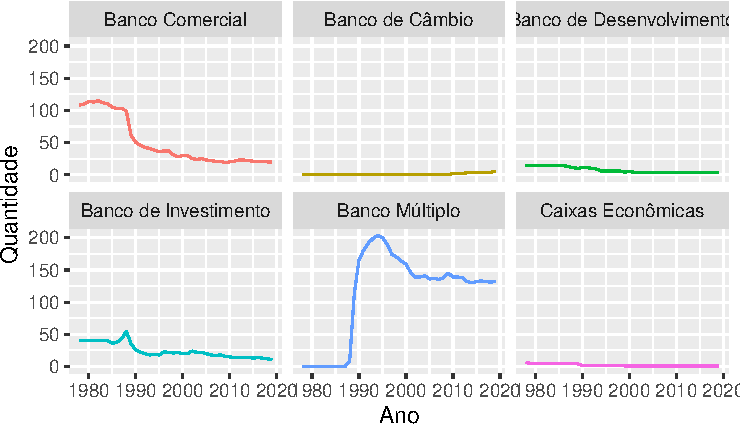
\includegraphics{12-exportedfigures/bank evolution-1} \end{center}

\label{fig:segmento}
\fonte{Desenvolvido pelo autor com dados do Banco Central}

O gráfico acima demonstra a evolução quantidade de instituições bancárias por segmento entre 1978 à 2019, podendo ser visualizada uma mudança na composição da estrutura, com significativos, aumento de instituições aderindo modalidades de múltiplas carteiras\footnote{As primeiras instituições com carteira múltipla começaram a operar no ano de 1988}, e redução de instituições que operavam exclusivamente com carteira comercial, e exclusivamente com carteira de investimento.

\begin{table}
\caption{Composição por tipo de iniciativa no setor bancário brasileiro — Dezembro 2019 }
\begingroup\fontsize{10}{12}\selectfont

\begin{tabu} to \linewidth {>{\raggedright\arraybackslash}p{8cm}>{\raggedright\arraybackslash}p{8cm}}
\toprule
Tipo & Participação\\
\midrule
\cellcolor{gray!6}{Privado} & \cellcolor{gray!6}{93\%}\\
Público & 7\%\\
\bottomrule
\end{tabu}
\endgroup{}
\label{tab:iniciativa}
\fonte{Desenvolvido pelo autor com dados do Banco Central}
\end{table}

Alguns dos efeitos da abertura comercial e financeira e das modificações na estrutura bancária provenientes das medidas governamentais foram o aumento da participação de instituições estrangeiras no país, e um consistente processo de fusões e aquisições, de ambas as origens de capital, que resultou em considerável elevação do grau de concentração \cite{camargo:2009}.

\captionof{figure}{Evolução da quantidade de instituições no setor bancário brasileiro}

\begin{center}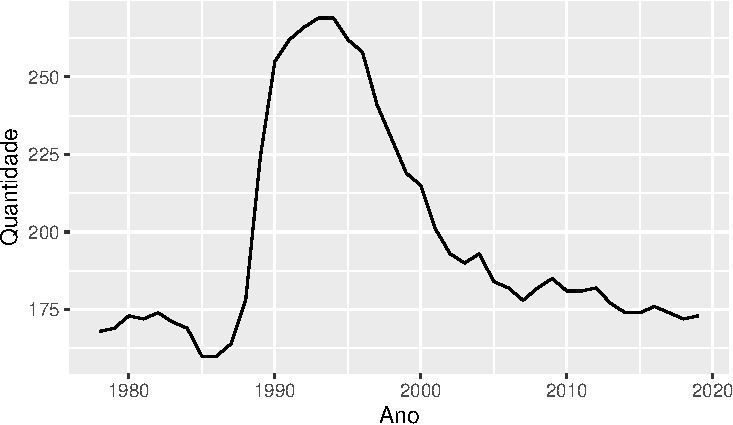
\includegraphics{12-exportedfigures/concetration-1} \end{center}

\label{fig:concentracao}
\fonte{Desenvolvido pelo autor com dados do Banco Central}

A observação sobre o aumento da concentração bancária no Brasil realizada por \textcite{camargo:2009} pode ser visualizada no gráfico acima. Entre as metades das décadas de 1980 e 1990 --- onde ocorreu o processo de abertura --- se visualizou uma redução da concentração, levando em consideração o número de instituições. Esse cenário passou se inverter a partir de 1994, chegando em 2019 a um nível aproximado ao observado no início da década de 1980.

De acordo com Strachman e Vasconcelos \emph{apud} \textcite{camargo:2009}, o aumento da concentração bancária pode ser prejudicial ao crescimento econômico, uma vez que, com maior participação de mercado, as instituições bancárias acabam por obter a prerrogativa de determinar seus preços, comportamento este observado em \textcite{klein:1971}.

Segundo \textcite{camargo:2009} por outra perspectiva, o ganho de escala, com redução de custos operacionais atua melhorando a remuneração dos depósitos podendo atuar na redução dos juros finais pagos pelos clientes.

Outra possível tendência para a concentração bancária é a redução do risco das operações, implicando em redução de custos, obtida por meio expansão geográfica, setorial e de produtos financeiros. Porém os possíveis efeitos da concentração dependem de uma série de condições, principalmente em torno da eficiência e do nível de concorrência no mercado \cite{camargo:2009}.

\begin{table}
\caption{Setor bancário brasileiro por origem de capital — Dezembro de 2019}
\begingroup\fontsize{10}{12}\selectfont

\begin{tabu} to \linewidth {>{\raggedright}X>{\raggedleft}X>{\raggedright}X}
\toprule
Capital & Quantidade & Participação\\
\midrule
\cellcolor{gray!6}{Nacionais} & \cellcolor{gray!6}{66} & \cellcolor{gray!6}{43.1\%}\\
Controle Estrangeiro & 60 & 39.2\%\\
\cellcolor{gray!6}{Nacionais com Participação Estrangeira} & \cellcolor{gray!6}{12} & \cellcolor{gray!6}{7.8\%}\\
Públicos & 10 & 6.5\%\\
\cellcolor{gray!6}{Estrangeiros} & \cellcolor{gray!6}{5} & \cellcolor{gray!6}{3.3\%}\\
\bottomrule
\end{tabu}
\endgroup{}
\label{tab:origemcapital}
\fonte{Desenvolvida pelo autor com dados do Banco Central}
\end{table}

\captionof{figure}{Evolução de origem de capital das instituições bancárias no Brasil}

\begin{center}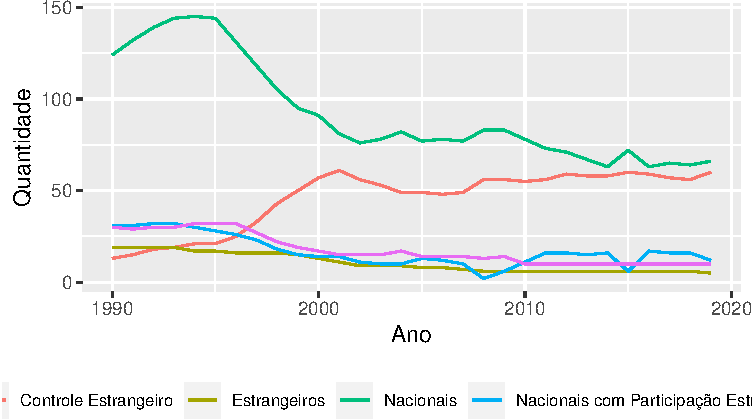
\includegraphics{12-exportedfigures/capital graphic-1} \end{center}

\label{fig: ev.capital}
\fonte{Desenvolvido pelo autor com dados do Banco Central}

O aumento da participação estrangeira no setor bancário brasileiro durante a década de 1990, evidenciado por \textcite{camargo:2009} pode ser observado no gráfico acima. Esse aumento ocorreu principalmente através do controle acionário, com elevação acentuada na segunda metade da década de 1990 até o início da década de 2000. Ocorrendo redução em instituições 100\% nacionais e estrangeiras e nacionais com participação estrangeira.

Durante este período, a inclinação para aplicação massiva em títulos públicas se dava diante a manutenção de elevadas taxas de juros, tornando o crédito para empreendimentos privados de elevado risco, e consequentemente elevando substancialmente o \emph{spread} bancário e reduzindo a oferta de crédito \cite{camargo:2009}.

A expectativa com a entrada de instituições estrangeiras era que houvesse elevação da concorrência e, consequentemente, redução no \emph{spread} bancário, aumento da concessão de crédito, melhoria da qualidade e diversificação do produtos financeiros, avanços em tecnologias, ou seja, uma elevação na eficiência do setor \cite{camargo:2009}.

Porém, o que se observou, de acordo com \textcite{camargo:2009}, foi a adoção de postura conservadora por partes dos bancos estrangeiros, com estratégia de ativos inclinada para negociação de títulos públicos, e passivos direcionados para a captação de recursos advindos de grupos de rendas média e alta, com exceção dos bancos públicos que concentraram em operações de crédito. O que levou a relação crédito/PIB ficar em níveis baixos comparados a outros países \cite{camargo:2009, leal:2006}.

Segundo Singh \emph{apud} \textcite{leal:2006}, durante a década de 1990 o \emph{spread} bancário no Brasil esteve superior a 50\%a.a., enquanto na América Latina esteve entre 10\% a 15\% a.a, e a relação crédito/PIB em 2003 no Brasil era de 23\%, muito abaixo de níveis considerados ótimos como: Chile com 68,5\%, Uruguai com 64,3\%, Estados Unidos com 60,8\%, Japão com 64,3\%, Coréia com 98,9\% e Europa com 140,6\%.

Durante o período citado, foi observado no setor bancário brasileiro os maiores níveis de \emph{spread} praticados no mundo, associado a um quadro econômico instabilidades e baixo crescimento e desenvolvimento. Esse cenário encontra embasamento em estudos teóricos e empíricos que demonstram que um sistema financeiro desenvolvido favorece o crescimento e desenvolvimento econômico \cite{levine:1997, matos:2003}.

\captionof{figure}{Evolução da relação Crédito/PIB no Brasil}

\begin{center}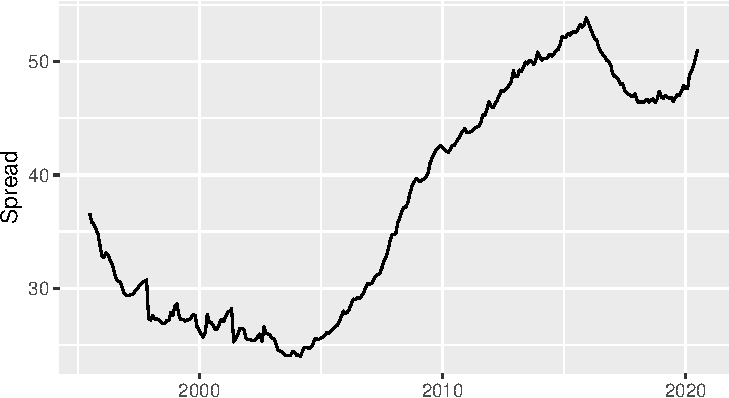
\includegraphics{12-exportedfigures/credit gdp-1} \end{center}

\label{fig:credgdp}
\fonte{Desenvolvido pelo autor com dados o Banco Central}

O gráfico acima demonstra o comportamento da relação crédito/PIB no Brasil, que entre a segunda metade da década de 1990 até a meados da primeira metade da década de 2000 sofreu significativa queda, ficando abaixo dos 25\%. Após esse período a oferta de crédito sofreu uma expansão exponencial atingindo patamares acima de 50\% do PIB.

\captionof{figure}{Evolução do \emph{spread} bancário brasileiro até 2011}

\begin{center}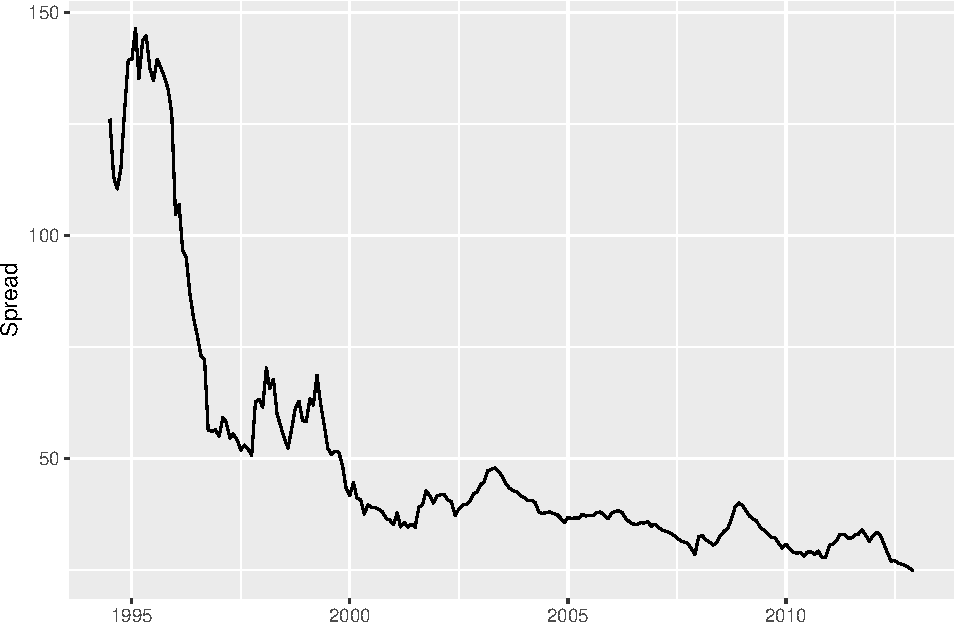
\includegraphics{12-exportedfigures/average spread-1} \end{center}

\label{fig:spread2012}
\fonte{Desenvolvido pelo autor com dados do Banco Central}

O gráfico acima mostra a evolução do \emph{spread} bancário brasileiro entre os anos de 1994 e 2012, saindo de patamares que chegaram próximo a 150\%, com significativa queda ao longo desse período, atingindo a casa de 25\% no final. Abaixo o gráfico visualiza a evolução do \emph{spread} entre 2012 e 2019, com nova metodologia de cálculo, chegando a ficar abaixo de 10\%, não ultrapassando a casa dos 23\% e terminando o período abaixo dos 18\%.

\captionof{figure}{Evolução do \emph{spread} bancário brasileiro entre 2012 e 2019}

\begin{center}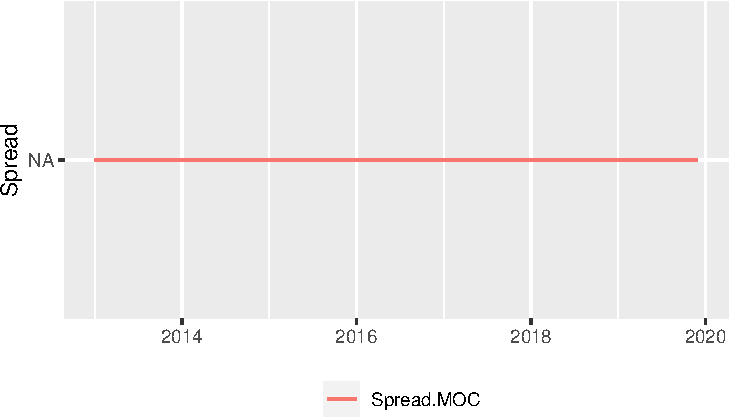
\includegraphics{12-exportedfigures/spread 2019-1} \end{center}

\label{fig:spread2019}
\fonte{Desenvolvido pelo autor com dados do Banco Central}

Diante o levantamento, o setor bancário brasileiro durante o período avaliado passou por diversas transformações em sua estrutura no que tange a concentração de mercado, aumento da participação de capital estrangeiro por meio de controle acionário, redução da participação pública.

Em relação aos indicadores foi verificado que entre a década de 1980 até metade da década de 1990, em um cenário hiperinflacionário, mesmo com redução da concentração bancária, os indicadores de eficiência de intermediação financeiras como o \emph{spread} bancário e a relação crédito/PIB estavam em níveis considerados ineficientes e muito destoantes em comparação a outros países e regiões.

A partir de 1995 se verificou mudanças significativas no setor bancário, com nova concentração, redução de instituições nacionais devido o controle acionário por capital estrangeiro, verificando queda expressiva no \emph{spread} bancário e a partir de 2004 uma mudança significativa na relação crédito/PIB.

Esse capítulo levantou informações amplas sobre o setor bancário brasileiro, e identificou como variáveis o nível de concentração, tipo de iniciativa, origem do capital, taxa de juros, \emph{spread} bancário, carteira de crédito de recursos livres e destinados, PIB\ldots{} No próximo capítulo serão levantadas conceitos e estudos sobre a decomposição e determinantes do \emph{spread} bancário.

\textual

\pagestyle{simple}

\chapter{Spread Bancário no Brasil}

Esse capítulo irá abordar sobre os conceitos, teorias do \emph{spread} bancário e os casos e estudos específicos para o cenário brasileiro. O foco é identificar elementos importantes que irão contribuir com o objeto deste estudo, assim como analisar os resultados dos estudos anteriores, verificando a complementariedade aos mesmos.

O \emph{spread} bancário é definido pela diferença, em pontos percentuais, entre a taxa de captação, que remunera as aplicações financeiras, e a taxa de aplicação incidente nas operações de crédito. No Brasil, a taxa de aplicação para crédito de recursos livres é pactuado entre instituição e tomadores. Somente as operações de crédito envolvendo recursos direcionados são sujeitas à limites, não podendo exceder 12\%a.a. mais a taxa referencial de juros \cite{BCB:2000}.

A margem de operação bancária é considerada um indicador de eficiência da economia, no sentido de favorecer o crédito e a atividade econômica. Em níveis elevados pode desfavorecer o crédito destinado a produção e consumo produtivos e estar associado com o fraco desempenho da economia \cite{WB:2005}.

O Banco Central, em 1999, iniciou uma série de estudos e medidas com objetivo de reduzir a taxa de juros e o \emph{spread} realizados no setor bancário brasileiro, atuando na identificação e ajustes em variáveis econômicas influentes. Entre as primeiras medidas estavam a redução da taxa de compulsório para depósitos à vista e até a extinção para depósitos à prazo, redução do IOF e a redução da Selic \cite{BCB:2000}.

Os estudos em torno do \emph{spread} bancário ocorrem em duas vertentes, a que visa definir sua estrutura e a que busca investigar seus determinantes. Em Dick \emph{apud} \cite{leal:2006} é destacada a importância de se distinguir a abordagem em torno da estrutura e determinante do \emph{spread} bancário, no sentido de complementariedade.

A abordagem em torno da estrutura para a margem bancária busca identificar e analisar os componentes de resultado envolvendo receitas e despesas. Enquanto a abordagem sobre os determinantes visam identificar as variáveis que explicam as variações do indicador ao longo dos períodos \cite{leal:2006}.

Vem se tornando relevantes os estudos em torno da decomposição do \emph{spread} bancário. Entre os componentes explícitos estão a inadimplência, despesas administrativas, impostos diretos e indiretos, e margem de lucro dos bancos. \cite{BCB:2000}. Essa configuração dos componentes, contemplando a margem de lucro vem desmistificar a comum abordagem do spread como o lucro dos bancos \cite{costa;nakane:2004}.

Além da avaliação de seus componentes, o \emph{spread} pode ser analisado conjuntamente por três características: enquanto a abrangência da amostra, conteúdo e origem da informação \cite{leal:2006}.

A abrangência da amostra consiste nas especificidades das operações de crédito das instituições e seu nível de agregação e granularidade \cite{costa;nakane:2004}. Uma análise agregada dessa característica pode ser dificultada pela existência de heterogeneidade do setor, ressaltando a importância de se realizar analises em diferentes características e óticas do \emph{spread} bancário. \cite{block:2000}.

O conteúdo está relacionado com os subcomponentes que envolvem a receita e as despesas das intermediações financeiras, podendo englobar ou não tarifas e comissões sobre as taxas de captações e aplicação \cite{block:2000}.

A origem da informação é analisada em dois cenários, o ex-ante e o ex-post \cite{kunt:1999}. A perspectiva ex-ante se refere a expectativa das instituições bancárias em relação aos riscos de mercado, considerando as taxas planejadas, basicamente resultado da diferença entre a taxa de captação e empréstimo. Essas informações são repassadas ao Banco Central que as divulgam \cite{durigan:2018}.

No cenário ex-post as margens são obtidas mediante a apuração dos resultados de contábeis, através dos demonstrativos, considerando as receitas e custos efetivos, implicando nas taxas realizadas \cite{kunt:1999, durigan:2018}.

Reduções no \emph{spread} ex-post não necessariamente significam aumento da eficiência da intermediação financeira, pois pode estar associada a uma redução da inadimplência \cite{kunt:1999}. Como observado em \textcite{klein:1971} e \textcite{ho-saunders:1981} o \emph{spread} bancário é determinado de acordo com as características e os riscos envolvidos nas intermediações financeiras inerentes em cada estrutura de mercado.

\section{Estudos anteriores}

Em \textcite{durigan:2018} foi realizada uma análise dos fatores macroeconômicos e indicadores industriais que influenciam o \emph{spread} bancário ex-ante, através de análise de regressão linear multivariada utilizando 18 variáveis em quatro modelos. Chegando a conclusão que o aumento da atividade industrial, a redução do desemprego e o consumo atuam na diminuição do \emph{spread} bancário.

Os modelos desenvolvidos por \textcite{durigan:2018} demonstraram que há uma uma significativa relação direta entre \emph{spread} e: inadimplência, IPIs (bens de capital, intermediários, semiduráveis, não duráveis e consumo duráveis), Selic, PIB, desemprego e o EMBI+ (medida de taxa de risco-país). As relações indiretas com o \emph{spread} foram encontradas: no IPI de bens de consumo e geral, IPCA, saldo da carteira de crédito e índice de vendas no varejo.

Em estudo dos determinantes macroeconômicos do \emph{spread} bancário ex-ante, \textcite{oreiro-2006} utilizou regressão múltipla para identificar as variáveis influentes. O estudo chegou ao resultado que alta volatilidade e as taxas da Selic são um dos principais determinantes desse indicador no setor bancário brasileiro, identificando também a significância do nível de atividade industrial.

\begin{table}
\caption{Resumo de Estudos sobre o *spread* bancário no brasil}
\begingroup\fontsize{10}{12}\selectfont

\begin{tabu} to \linewidth {>{\raggedright\arraybackslash}p{1cm}>{\raggedright\arraybackslash}p{3cm}>{\raggedright\arraybackslash}p{12cm}}
\toprule
Método & Autores & Variáveis.Explicativas\\
\midrule
\cellcolor{gray!6}{Ex-ante} & \cellcolor{gray!6}{KOYAMA e NAKANE (2001a e 2001b)} & \cellcolor{gray!6}{Selic (+); spread over treasury (+); impostos indiretos (+); custo administrativo (+); IGP(+); Produto industrial (–); Requerimento de reserva (+).}\\
Ex-ante & AFANASIEFF, LHAGER e NAKANE (2001 e 2002) & Custo operacional (+); captação sem custo de juros (+); receita de serviços (+); IGP (+); crescimento do produto industrial (–); Selic (+); volatilidade da Selic (–); banco estrangeiro (–); IGP (–); cresci- mento do produto industrial (+); spread over treasury (+); impostos indiretos (+).\\
\cellcolor{gray!6}{Ex-ante} & \cellcolor{gray!6}{BIGNOTTO e RODRIGUES (2006)} & \cellcolor{gray!6}{IPCA (–); Selic (+); custo administrativo (+); risco de juros (+); risco de crédito (+); parcela de mercado (–); liquidez (+); receita de serviços (+); compulsório (+); ativo total (+),.}\\
Ex-ante & OREIRO et al. (2006) & Produto industrial (+); Selic (+); volatilidade da Selic (+).\\
\cellcolor{gray!6}{Ex-Post} & \cellcolor{gray!6}{GUIMARÃES (2002)} & \cellcolor{gray!6}{Participação dos bancos estrangeiros (+); caixa e depósitos (+).}\\
\bottomrule
\end{tabu}
\endgroup{}
\label{tab:estudos}
\fonte{\cite{dantas:2012}}
\end{table}

De acordo com \textcite{durigan:2018, dantas:2012}, existem poucos estudos inclinados para os determinantes do \emph{spread} ex-post no Brasil, que identificaram o estudos de Guimarães (2002). Foram identificados ainda os estudos acerca do \emph{spread} ex-pots de Fipecafi (2004) \emph{apud} \textcite{dantas:2012} e Matias (2006) \emph{apud} \textcite{leal:2006}

Em análise dos determinantes do \emph{spread} bancário ex-post, \textcite{dantas:2012} utilizaram variáveis explanatórias microeconômicas de cada instituição, por meio de dados em painel dinâmico, entre janeiro de 2000 e outubro de 2009, encontrando níveis significativos e diretos com o risco de crédito, grau de concentração e nível de atividade econômica, e indireta com a participação da instituição no mercado, não encontrando níveis significativos com origem de capital, e tipo de organismo.

Outra observação em \textcite{dantas:2012} foi a forte relação do \emph{spread} ex-post no momento atual com o momento anterior imediato, e que as instituições tendem a cobrar maiores taxas, quando maior o nível de concentração do mercado, não encontrando significância da Selic na determinação nesse indicador.

O estudo de \textcite{timotio:2018} teve foco em uma abordagem microeconômica ao buscar identificar a influência das variações de indicadores financeiros-contábeis no \emph{spread} bancário em 26 instituições bancárias, através de regressão em dados em painel. Encontrado uma relações significativas diretas com a alavancagem financeira, retorno sobre o patrimônio líquido, EBITDA, Ativo Total e eficiência.

No modelo de \textcite{timotio:2018} foi encontrada relação significativa e indireta do \emph{spread} com a participação de capital de terceiros, e não identificada relação significativa com a composição do endividamento, Retorno sobre ativos e a liquidez corrente.

\part{Desenvolvimento}

\chapter{Metodologia}

\chapter{Aplicação}

\chapter{Resultados}

\phantompart

\chapter*[Conclusão]{CONSIDERAÇÕES FINAIS}
\addcontentsline{toc}{chapter}{CONSIDERAÇÕES FINAIS}

\postextual

\addtocontents{toc}{\vspace{-2pt}}

\SingleSpacing

\printbibliography

\postextual

\addtocontents{toc}{\vspace{-2pt}}

\ifthenelse{\equal{\terApendice}{Sim}}
{\begin{apendicesenv}

\renewcommand{\thechapter}{\arabic{chapter}}

\chapter{Replicação de Estudos}
\section{}
 
\end{apendicesenv}
}{}

\ifthenelse{\equal{\terAnexo}{Sim}}{
\begin{anexosenv}

\renewcommand{\thechapter}{\arabic{chapter}}
        
\chapter{Cálculo Resultados}

\lipsum[31] 

\lipsum[32] 

\end{anexosenv}
}{}

\ifthenelse{\equal{\terIndiceR}{Sim}}{
\phantompart
\printindex
}{}

\printbibliography

\end{document}
